\color{red}
Firstly we cover the technical advances in object detection over the past decade and its usage in traffic monitoring.
\color{black}

% --------------------------------------------------------------------------------------
\color{red}
\subsection{Inclusive infrastructure}
Why it is crucial to understand cyclist behavior, and especially in cities with emerging bike infrastructure, \textit{how they adapt}.
We focus on the psychological aspects of a cyclist,

\begin{itemize}
	\item Perception of safety
	\item Intuitiveness (right-of-way should be obvious)
	\item Congestion (incl. waiting times)
	\item Rule compliance
\end{itemize}

If new cyclists feel uncomfortable (stress, embarrassment, etc.) they are more likely to give up on the bike. This leaves the infrastructure 
under-used, which can further result in a back-clash against "bike culture". 
\ \\

\color{black}
 % -----------------------------------------------------------------------------------
\subsection{Staging mobilities}
The book 'Designing Mobilities' (\cite{designinig_mobilities}) explores \textit{what physical, social, technical, 
and cultural conditions contribute to the staging of contemporary urban mobilities?} 
It covers how to capture and represent \textit{mobilities} and flows by presenting a theoretical framework for 'staging mobilities'. 
Most importantly it introduces a set of concepts for articulating \textit{situational perspectives}, 
including the two metaphors \textit{the river} and \textit{the ballet}. 
 \ \\

 The \textit{river} references the notion of capturing mobility from a 'birds-eye view' including the layout, 
 flows, and obstacles of a location, and hence, can be interpreted as a 'flowing riverbed'. 
 From this perspective, we can observe road users' behavior in aggregate and as part of more significant 'streams'. 
 This can be used to encapsulate abstract and high-level features of cyclists, such as the change in paths
 when infrastructure is changed or when temporary obstacles come along (e.g., road work).
 \ \\

In contrast, the \textit{ballet} is the micro-perspective, encompassing the gestures and small interactions at the individual level.
This perspective is an important supplement to the former \textit{river} as subtle interactional patterns which can, for instance,
 signal agreement or evasion.

 % -----------------------------------------------------------------------------------
\subsubsection{Case studies}
\textit{Study of mobilities in 'situ'} (\cite{situ}) uses the above framework as part of a case study involving cycling infrastructure in 
Copenhagen and Amsterdam. Quantitative data (as part of the \textit{river} perspective) was obtained by filming cyclists and conducting 
"desire lines analysis" (\cite{cva}) to gain a structured overview of the behavior of cyclists and intersections. 


 % -----------------------------------------------------------------------------------

 While on-site assertion of an intersection is plausible, the scope of a single observer is limited, as one can only keep track of 
 so many cyclists at once. Likewise, while not bounded by time, analyzing recorded video footage is still a time-consuming process, 
 especially as the views of cyclists can be obstructed by other passing vehicles or permanent installations.
\ \\

The latter issue of keeping track of unique cyclists as their view is temporally obstructed is one also faced by 
object tracking algorithms in video. We therefore propose deploying a multi-camera setup, overlooking the intersection from
multiple sides.

In theory, a top-down overhead view, overlooking from the center of the intersection would be optimal for minimizing obstruction.
The height required for such a recording setup as well as lack of permanent fixtures makes this approach very impractical. 
Further, current state-of-the-art object detection algorithms (e.g. YOLO) perform worse at catecorising objects, especially bicycles, 
using an overhead view compared to a semi-frontal view.

Pragmatic approach


\subsection{OpenDataCam}
OpenDataCam (ODC) is an exsisting open-source tool for processing video footage from urban environments to quantify
*URABN environments*. The novelty of OpenDataCam is that it is designed for the on-site, real-time processing of video. 
This requires dedicated CUDA-enabled hardware such as an Nvidia Jetson series of devices. 
\ \\

The backbone of the application is based on Darknet with YOLOv4 as the model used for detecting objects in video.
\href{https://pjreddie.com/darknet/yolo/}{YOLO}, \textit{You Only Look Once}, is a real-time object detection algorithm. 
YOLO is trained on the \href{https://cocodataset.org}{COCO dataset}, which comprises over 330,000 thousand images
with over 1,5 million objects in over 80 object classes, including cars, people and cyclists. 
YOLO is well known for its real-time speed and accuracy (\cite{redmon2016look}).
\ \\

The user interacts with the application through a web interface which displays a live preview of the footage with
indicators around all detected objects.

\ \\
\raggedbottom
\noindent
\begin{tabular}{@{}cc}
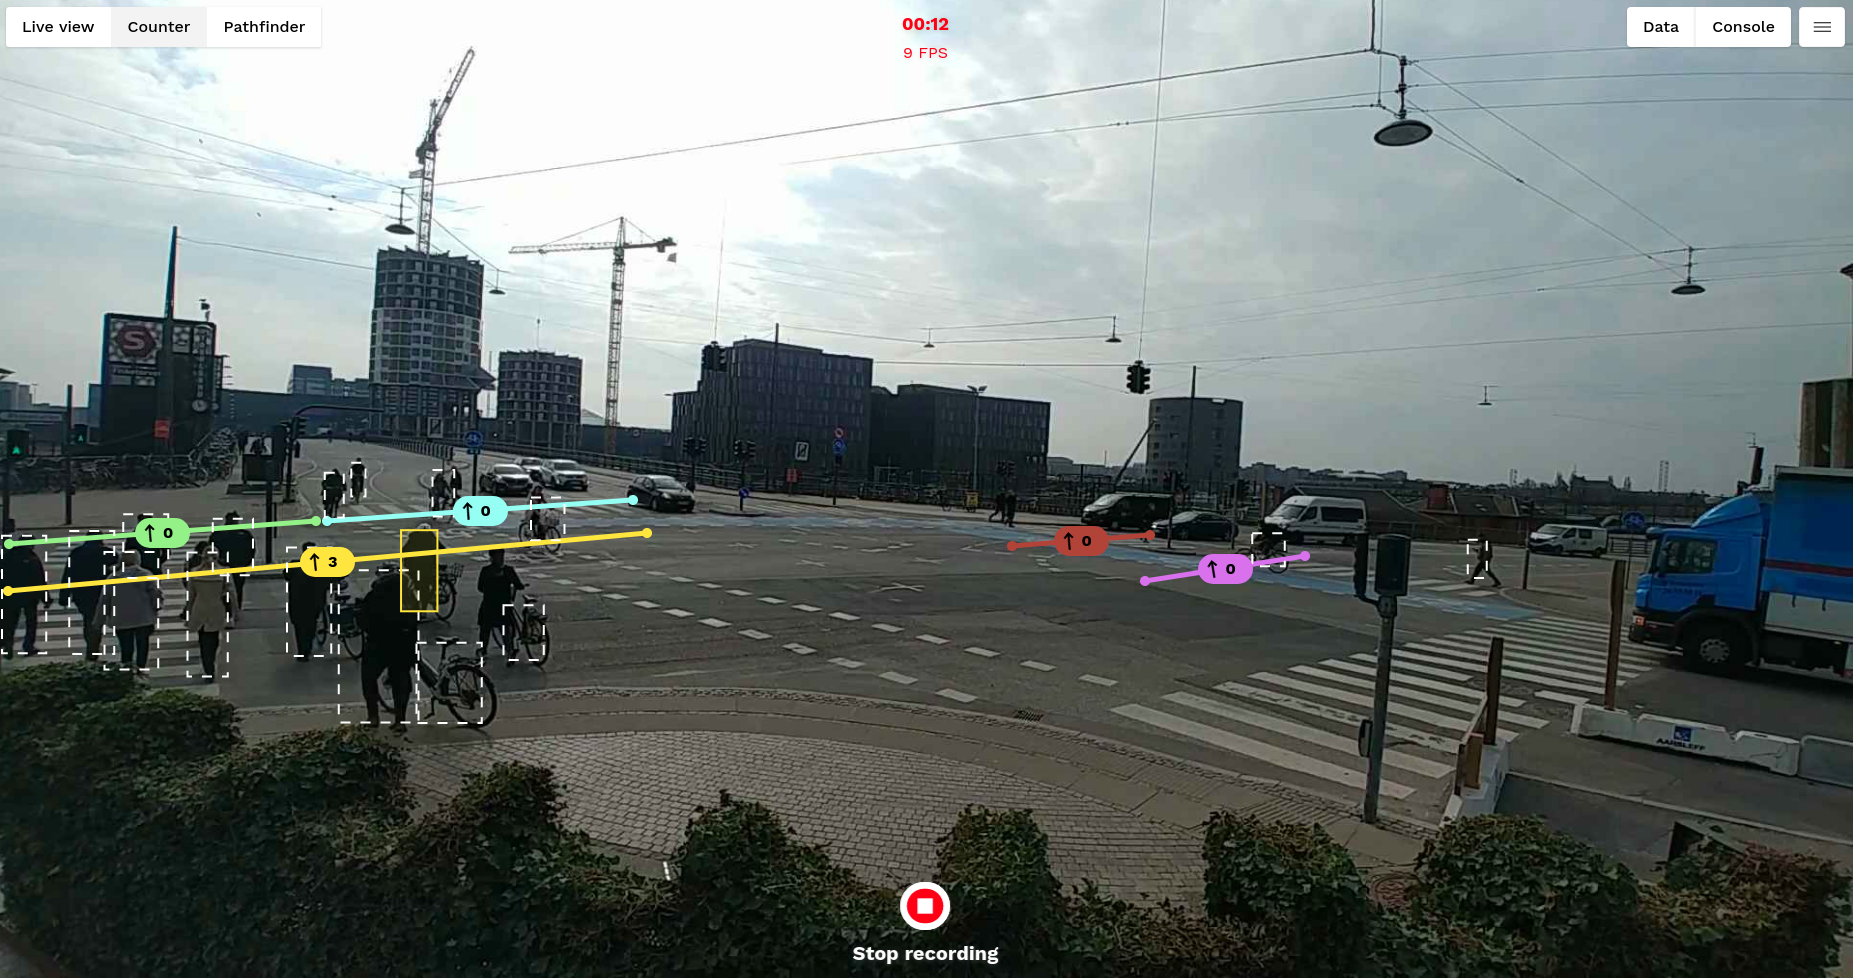
\includegraphics[width=1.0\columnwidth]{odc} 
\end{tabular}
\captionof{figure}{OpenDataCam web interface}
\ \\

Using the interface, a user can draw counting lines, which, when passed by a detected object at a certain angle, 
increments a counter. Apart from counting functionality, the app also offers the trajectories of uniquely identified objects. 

\raggedbottom
\subsubsection{Application}
As a baseline, we deployed an OpenDataCam setup using pre-recorded footage from the Dybbølsbro intersection in Copenhagen.
Our goal was to extract pre-defined desire lines using the counting line functionality. We did this by drawing an inital 
'base line' followed two (or more) additional counting lines, which allow us to branch cyclists into multiple segments. Inspecting the
overlap of unique cyclists who have passed both the base line and one (or more) of the branching lines would thus yield which path
they took. 
\ \\

\color{red}
Insert graphic here :) 
\color{black}
\ \\

However, this approach was limited by the poor performance of the detection of cyclists implemented in the current 
version of OpenDataCam (YOLOv4). Due to the intermittent detection of cyclists, the tracking algorithm would constantly 
re-identify the same cyclists as new ones. Thus, even when the same cyclists passed both the 'base line' and one of the 
branching lines, they wouldn't be included in desire line. Hence, not useful :(
\ \\

We will discuss the findings derived from OpenDataCam on our own case study in later sections of the report.
